\documentclass[11pt,letterpaper]{article}
\PassOptionsToPackage{hyphens}{url}
\usepackage[margin=.83in,top=.8in,bottom=.8in,headheight=15pt]{geometry}
\usepackage[T1]{fontenc}
\usepackage{lmodern,amsmath,amssymb,mathtools,bm,booktabs,array,graphicx,tikz}
\usetikzlibrary{arrows.meta,positioning,calc,decorations.pathreplacing,patterns}
\definecolor{ink}{HTML}{17344D}\definecolor{accent}{HTML}{087E8B}\definecolor{pale}{HTML}{EDF5F5}\definecolor{gold}{HTML}{AD6B19}
\providecommand{\dd}{\,\mathrm{d}}\providecommand{\R}{\mathbb{R}}
\providecommand{\E}{\mathbb{E}}\providecommand{\Var}{\operatorname{Var}}
\providecommand{\Cov}{\operatorname{Cov}}\providecommand{\diag}{\operatorname{diag}}
\providecommand{\norm}[1]{\left\lVert#1\right\rVert}
\providecommand{\abs}[1]{\left|#1\right|}
\usepackage{microtype,hyperref,fancyhdr,enumitem,amsthm,sectsty,needspace}
\allsectionsfont{\raggedright}
\hypersetup{colorlinks=true,linkcolor=ink,urlcolor=accent,pdfauthor={Zan Ahmad},pdftitle={ODE integration, root finding, and parameter estimation / Lecture notes}}
\setlength{\parindent}{0pt}\setlength{\parskip}{6pt}\linespread{1.07}
\setlist{itemsep=3pt,topsep=4pt,leftmargin=*}
\emergencystretch=2em\clubpenalty=10000\widowpenalty=10000
\pagestyle{fancy}\fancyhf{}\fancyhead[L]{\small Scientific Computing in Python}\fancyhead[R]{\small Lecture 4}
\fancyfoot[L]{\footnotesize Zan Ahmad}\fancyfoot[R]{\footnotesize\thepage}\renewcommand{\headrulewidth}{.3pt}
\newtheorem{proposition}{Proposition}\newtheorem{theorem}{Theorem}\newtheorem{lemma}{Lemma}
\theoremstyle{definition}\newtheorem{definition}{Definition}\newtheorem{example}{Example}
\numberwithin{equation}{section}
\begin{document}
{\small\scshape Scientific Computing in Python\hfill Lecture 4}\par\medskip
{\raggedright\hyphenpenalty=10000\exhyphenpenalty=10000\LARGE\bfseries\color{ink} ODE integration, root finding, and parameter estimation\par}\medskip
{\small Lecture notes}\par\bigskip
Newton's cooling law provides one model on which to compare several numerical operations. We derive the exact solution first. It then supplies a reference for an ODE solver, a threshold-time calculation, interpolation, and a parameter fit. Each operation has its own input and its own source of error.

\section{Newton's cooling equation}
\hypertarget{note-newton-s-cooling-equation}{}\label{note:newton-s-cooling-equation}
{\small \href{slides.html\#frame=newton-s-cooling-equation\&step=1}{Slides for this section}}\par
Assume a well-mixed body, constant ambient temperature $T_a$, and a constant heat-transfer coefficient represented by $k>0$. The rate of temperature change is proportional to the difference from ambient. The model treats the ambient environment as an effectively fixed reservoir.

\[
\dot T=-k(T-T_a),\qquad T(0)=T_0.
\]

Set $u=T-T_a$. Then $\dot u=-ku$, and $k$ has units of inverse time.

\subsection*{Exact solution}
\[
\frac{\dd u}{u}=-k\,\dd t
\quad\Longrightarrow\quad
\log\left|\frac{u(t)}{u(0)}\right|=-kt.
\]

\[
T(t)=T_a+(T_0-T_a)e^{-kt}.
\]

The separation step assumes $u(0)=T_0-T_a\ne0$. If $T_0=T_a$, the solution is the constant $T(t)=T_a$, also included in the final exponential formula.
\section{Time scales and forward Euler}
\hypertarget{note-time-scales-and-forward-euler}{}\label{note:time-scales-and-forward-euler}
{\small \href{slides.html\#frame=time-scales-and-forward-euler\&step=1}{Slides for this section}}\par
The relaxation time is $\tau=1/k$. Over one relaxation time the temperature difference is multiplied by $e^{-1}$. Euler's method replaces the derivative by a forward difference. Its behavior is controlled by the dimensionless step $kh$, rather than by the step length alone.

\[
T_{n+1}=T_n-hk(T_n-T_a),\qquad
u_{n+1}=(1-kh)u_n.
\]

Decay requires $|1-kh|<1$, or $0<kh<2$.

\subsection*{Monotone versus oscillatory decay}
\[
0<kh\leq1:\quad u_n\text{ preserves sign and decays},
\]

\[
1<kh<2:\quad u_n\text{ alternates sign while decaying}.
\]
The second behavior is numerically stable but inconsistent with monotone cooling in this model.
\section{Adaptive integration}
\hypertarget{note-adaptive-integration}{}\label{note:adaptive-integration}
{\small \href{slides.html\#frame=adaptive-integration\&step=1}{Slides for this section}}\par
An adaptive solver chooses internal steps to keep a local error estimate within an absolute-plus-relative tolerance. Requested output times are not generally the solver's internal step times. Successful termination indicates that the algorithm met its stopping conditions; accuracy should still be compared with the known reference in this example.

\begin{minipage}{\linewidth}
\begin{verbatim}
sol = solve_ivp(rhs, (0, 8), [80],
                t_eval=times, rtol=1e-8, atol=1e-10)
\end{verbatim}
\end{minipage}

Compare $T_{\rm num}(t_i)$ with $20+60e^{-0.4t_i}$.

\subsection*{Error under refinement}
\[
E(h)=\max_i|T_h(t_i)-T(t_i)|.
\]

For first-order Euler convergence, $E(h)/E(h/2)$ approaches $2$ when the step is sufficiently small and roundoff does not dominate.
\begin{center}\begin{minipage}{.98\linewidth}\centering
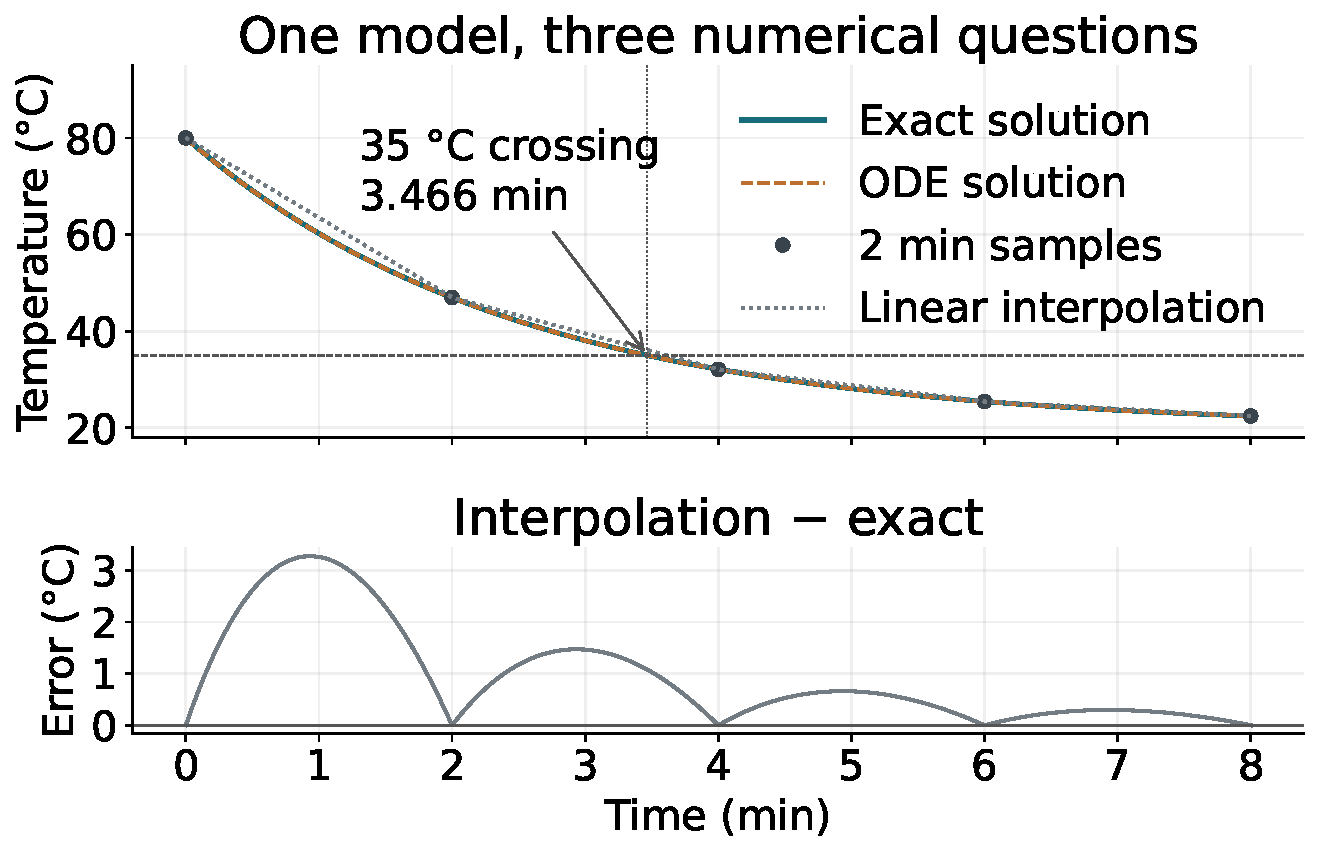
\includegraphics[width=.96\linewidth,height=.57\textheight,keepaspectratio]{cooling-questions.pdf}\par\smallskip
{\small The ODE and exact solution use k =\allowbreak{} 0.4 per minute, initial 80 degrees Celsius and ambient 20 degrees. Linear interpolation uses samples every two minutes; its discrepancy is shown below.}
\end{minipage}\end{center}
\section{Threshold time as a root}
\hypertarget{note-threshold-time-as-a-root}{}\label{note:threshold-time-as-a-root}
{\small \href{slides.html\#frame=threshold-time-as-a-root\&step=1}{Slides for this section}}\par
A crossing time solves $g(t)=T(t)-T_*=0$. For cooling from above ambient, a finite positive crossing occurs when $T_a<T_*<T_0$. A bracketed root method uses continuity and opposite endpoint signs. The exact formula allows the numerical root to be checked independently.

\[
T_*-T_a=(T_0-T_a)e^{-kt_*}.
\]

\[
t_* =\frac1k\log\frac{T_0-T_a}{T_*-T_a}.
\]

\subsection*{A threshold calculation}
For $T_0=80$, $T_a=20$, $k=0.4$ and $T_*=40$,
\[
t_* =2.5\log3\approx2.74653\ \mathrm{min}.
\]

The logarithm's argument is dimensionless and greater than one.
\section{Linear interpolation}
\hypertarget{note-linear-interpolation}{}\label{note:linear-interpolation}
{\small \href{slides.html\#frame=cooling-trajectory-and-interpolation-error-figure\&step=1}{Slides for this section}}\par
Between two sampled values, linear interpolation assumes a constant secant slope. It reproduces the endpoints exactly, but it does not reproduce a curved solution between them. For a twice differentiable function its local error is proportional to the curvature and the product of the distances to the endpoints.

\[
\widetilde T(t)=(1-\alpha)T_i+\alpha T_{i+1},\qquad
\alpha=\frac{t-t_i}{t_{i+1}-t_i}.
\]

Here $0\leq\alpha\leq1$ only within the sampled interval.

\subsection*{Interpolation error for cooling}
\[
T(t)-\widetilde T(t)=\frac{T''(\xi)}2(t-t_i)(t-t_{i+1}).
\]

Cooling from above ambient has $T''>0$. The product is nonpositive inside the interval, so the secant lies above the exact curve.
\begin{center}\begin{minipage}{.98\linewidth}\centering
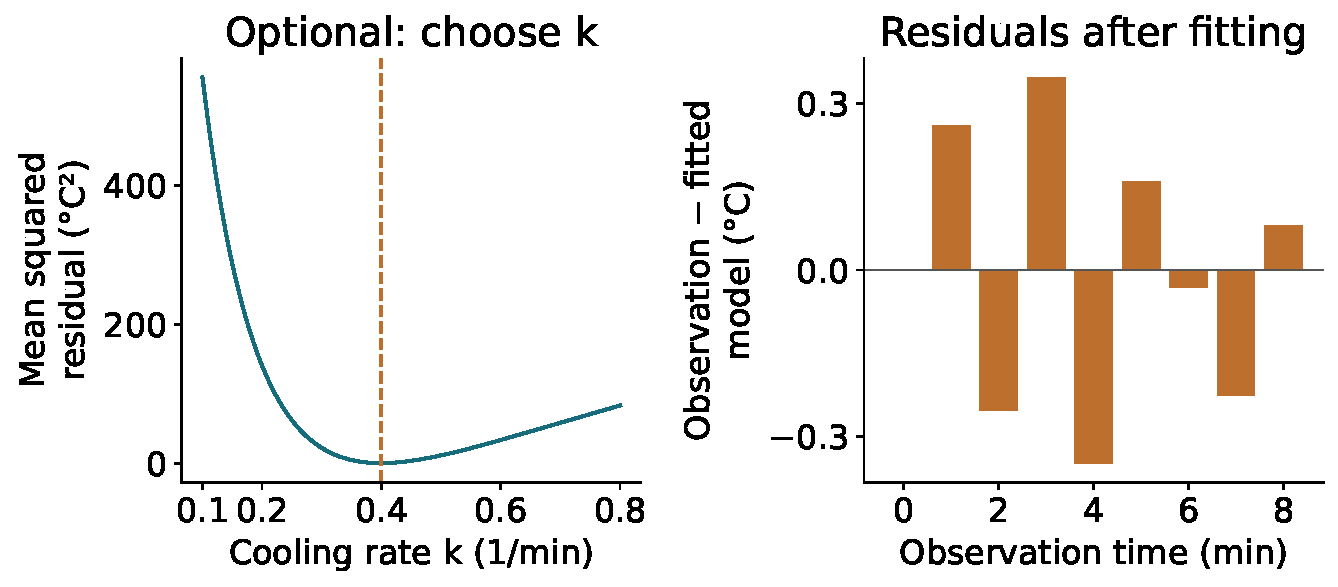
\includegraphics[width=.96\linewidth,height=.57\textheight,keepaspectratio]{fit-and-residuals.pdf}\par\smallskip
{\small Nine synthetic perturbed observations define a mean-squared residual objective. The chosen parameter leaves residuals; fitting does not validate the physical model.}
\end{minipage}\end{center}
\section{Fitting the cooling coefficient}
\hypertarget{note-fitting-the-cooling-coefficient}{}\label{note:fitting-the-cooling-coefficient}
{\small \href{slides.html\#frame=parameter-objective-and-residuals-figure\&step=1}{Slides for this section}}\par
With observed temperatures $y_i$, define residuals $r_i(k)=T(t_i;k)-y_i$ and minimize their squared sum. Numerical integration error, observation error, and model discrepancy are separate contributions. Bounds on $k$ constrain the fit but do not prove that the physical cooling model is adequate.

\[
J(k)=\frac1n\sum_i[T_a+(T_0-T_a)e^{-kt_i}-y_i]^2.
\]

\[
\frac{\partial T(t;k)}{\partial k}=-t(T_0-T_a)e^{-kt}.
\]

\subsection*{Sensitivity in time}
At $t=0$, the temperature is independent of $k$. At very long times it is nearly ambient and again weakly sensitive.

For $t>0$, the magnitude $te^{-kt}$ is largest at $t=1/k$. Measurements near that scale are informative about $k$.
\bigskip
\section*{Exercises}
\par\noindent\begin{minipage}{\linewidth}
\subsection*{H4-1. Check a new cooling model}
Use ambient 18 degrees Celsius, initial 58 degrees Celsius and k =\allowbreak{} 0.25 per minute. New practice; 10 feedback points.

\textbf{a} Write the rate law and exact solution, with units for k.

\end{minipage}\par\medskip
\textbf{b} Find the initial temperature-change rate and the temperature at four minutes.

\textbf{c} Give one zero-rate check and one long-time check that do not depend on a solver success flag.

\par\noindent\begin{minipage}{\linewidth}
\subsection*{H4-2. Form and audit a crossing-time calculation}
Use the model from H4-1 and target 28 degrees Celsius. New practice; 10 feedback points.

\textbf{a} Define the scalar residual and show that [0, 8] minutes brackets a root.

\end{minipage}\par\medskip
\textbf{b} Calculate the exact crossing time and describe how to check a numerical result.

\textbf{c} Explain why targets of 18 and 16 degrees do not have finite future crossings in this model.

\par\noindent\begin{minipage}{\linewidth}
\subsection*{H4-3. Separate interpolation from a model prediction}
Two samples are 50 degrees Celsius at minute 1 and 32 degrees at minute 4. No rate law is given. New practice; 10 feedback points.

\textbf{a} Use piecewise linear interpolation to estimate the temperature at minute 2, and state the interpolation weight.

\end{minipage}\par\medskip
\textbf{b} What do the two samples establish, and what extra assumption produced the value at minute 2?

\textbf{c} Explain why the supplied wrapper rejects a query at minute 5 and why returning 32 would require explanation.

\par\noindent\begin{minipage}{\linewidth}
\subsection*{H4-4. Optional new optimization extension}
This exercise is outside the core 150-minute allocation. For a fixed model, three candidate k values have residuals in degrees Celsius: k =\allowbreak{} 0.2 gives [2, -1]; k =\allowbreak{} 0.3 gives [1, -1]; k =\allowbreak{} 0.4 gives [0, -2]. New practice; 10 feedback points.

\textbf{a} Compute the mean squared residual for each candidate and select the best of these three.

\end{minipage}\par\medskip
\textbf{b} Does that selection prove the globally best continuous parameter or validate the model? Explain both limits.

\textbf{c} Describe a synthetic parameter-recovery check and explain what it can establish.

\section*{References}
\noindent\begin{minipage}{\linewidth}
Original Python Lecture 4. PDF pages 4--17.

\url{https://zanahmad.com/files/scientific-python/Lecture_4__Intro_to_Python.pdf}
\end{minipage}\par\medskip
\noindent\begin{minipage}{\linewidth}
SciPy solve\_ivp reference. Parameters fun, t\_span, y0, t\_eval, rtol/atol; returned success and y.

\url{https://docs.scipy.org/doc/scipy/reference/generated/scipy.integrate.solve_ivp.html}
\end{minipage}\par\medskip
\noindent\begin{minipage}{\linewidth}
SciPy brentq reference. Continuity and bracketing requirements; xtol; RootResults.

\url{https://docs.scipy.org/doc/scipy/reference/generated/scipy.optimize.brentq.html}
\end{minipage}\par\medskip
\noindent\begin{minipage}{\linewidth}
NumPy interp reference. One-dimensional linear interpolation; increasing xp; endpoint behavior.

\url{https://numpy.org/doc/stable/reference/generated/numpy.interp.html}
\end{minipage}\par\medskip
\noindent\begin{minipage}{\linewidth}
SciPy minimize\_scalar reference. Optional extension: bounded method, bounds and success.

\url{https://docs.scipy.org/doc/scipy/reference/generated/scipy.optimize.minimize_scalar.html}
\end{minipage}\par\medskip
Python source materials: Phillip Kerger (2023). Course adaptation and additional exposition: Zan Ahmad.

\end{document}
